\documentclass{article}

\title{The influence of voluntary actions on temporal preparation to visual stimuli}
\author{Alexandre de Pontes Nobre, André Mascioli Cravo}

\usepackage[a4paper, margin=1in]{geometry}
\usepackage[backend=biber, style = apa]{biblatex}
%\usepackage{natbib}
\usepackage{graphicx}
\usepackage{amsmath}
\usepackage{soul} % for highlighting


\addbibresource{bibliography.bib}

\usepackage{Sweave}
\begin{document}
\Sconcordance{concordance:action_foreperiod_paper.tex:action_foreperiod_paper.Rnw:%
1 15 1 1 0 77 1}


\maketitle

\section{Experiment 1}

\graphicspath{{./Figures/Exp_1/}}

\subsection{Methods}

\subsubsection{Participants}
Thirty-seven volunteers were recruited to participate in the study. All reported normal or corrected-to-normal vision and no history of neurological disorders, and none had any knowledge of the purpose of the study before the experiment. All participants read and signed an informed consent. The experimental protocol was approved by the research ethics committee of the Federal University of ABC. Two participants were removed from the analysis due to a large number of errors (> 10\% of trials), resulting in a final sample size of 35 participants.


\subsubsection{Stimuli and procedure}
The experiment was conducted online on Pavlovia. Participants received the instructions and the link to the experimental after reading and signing the informed consent. They were instructed to sit quietly in a place free of distractions when performing the task.

Figure 1 shows an experimental trial. Each trial started with a black fixation cross presented at the center of the screen. The fication cross remained on the screen for a period depending on the experimental condition. In the \textit{external} condition, the fixation cross remained on the screen for an interval of 1250-1750 ms (uniformly distributed), after which the warning signal (WS) was presented automatically. In the \textit{action} condition, the fixation cross remained on the screen until the participant pressed the space bar, which they could do whenever they desired. After either the fixation time or the voluntary action by the participant, the fixation changed color from black to green; this change was the WS and marked the onset of the FP. FP duration was either 600, 1200 or 1800 ms, and was pseudorandomly sampled from a uniform distribution in each trial, with the constraint the all durations were presented for an equal number of trials within a block. After the FP had elapsed, the fixation cross was replaced by the target: an imperative stimulus, which was either a go or no-go stimulus, as shown in Figure 1. Participants were instructed to press the space bar if they saw a go stimulus, or refrain from pressing any key if the saw a no-go stimulus. The target remained on the screen for 200 ms, and participants had up to 1000 ms to respond. After the response window, a blank screen was presented during a intertrial interval (ITI) drawn from a gaussian distribution with mean = 250 ms and sd = 25 ms. % min = 160 ms, max = 330 ms

% Insert figure 1 here

The experiment comprised four blocks of 75 trials, two for each condition (action vs. external). Within blocks, 80\% of trials were go trials, and 20\% were no-go trials. The order of the conditions was counterbalanced across participants, and blocks of different conditions could not be intermixed. Each condition started with a practice block of six trials for that condition, with three trials for each FP duration (600, 1200, and 1800 ms) and trial type (go vs no-go).


\subsubsection{Data analysis}
We analyzed accuracy (proportion of correct responses) and reaction time (RT) separately for each participant, condition, foreperiod and, for accuracy, trial type. For RT, only correct trials were included in the analysis. Participants with over 10\% of incorrect responses were removed from the analysis. Additionally, RTs more than 3 standard deviations away from the participant's mean RT were discarded \hl{insert mean and sd discarded}.
For RT, we first conducted a three-way repeated measures ANOVAs with the factors foreperiod in the current trial (FP\textsubscript{n}), foreperiod in the previous trial (FP\textsubscript{n-1}), and condition.

Additionally, we examined the fits of the data by each participant. We observed considerable variability in slopes across participants (supplemental figure 1), which led us to fit mixed models \hl{description}.

Finally, a previous study \cite{los_role_2013} found that no-go trials increased the magnitude of sequential for short durations of (FP\textsubscript{n}). To examine the impact of no-go trials in our design we ran the same ANOVAs as above including the trial type (go vs no-go) on trial n-1.

\subsubsection{Results}
Figure 2 shows the RT curves by FP duration and condition. We tested for differences between these conditions with a repeated-measures ANOVA. Mauchly's test of sphericity showed a violation for FP\textsubscript{n} (\textit{p} = 0.025), FP\textsubscript{n-1} (\textit{p} = 0.009), and the three-way interaction between FP\textsubscript{n}, FP\textsubscript{n-1} and condition (\textit{p} = 0.013), so the Greenhouse-Geisser correction was applied. We found main effects of FP (\textit{F}(1.66, 56.61) = 84.01, \textit{p} < .001, $\eta_{p}^{2}$ = .712), condition (\textit{F}(1, 34) = 4.80, \textit{p} = .035, $\eta_{p}^{2}$ = .124), and FP\textsubscript{n-1} (\textit{F}(1.85, 62.90) = 31.61, \textit{p} < .001, $\eta_{p}^{2}$ = .482). The main effect of FP\textsubscript{n} was moderated by an interaction between FP\textsubscript{n} and condition (\textit{F}(1.95, 66.32) = 23.25, \textit{p} < .001, $\eta_{p}^{2}$ = .406). Follow-up pairwise comparisons using the Holm correction for p-values showed that RTs were systematically higher for FP\textsubscript{n} = 600 ms (\textit{t}(34) = 3.82, \textit{p} = .0005), but not for FP\textsubscript{n} = 1200 ms (\textit{t}(34) = 1.71, \textit{p} = .10) or FP\textsubscript{n} = 1800 ms (\textit{t}(34) = 0.26, \textit{p} = .80).


\begin{figure}[h]
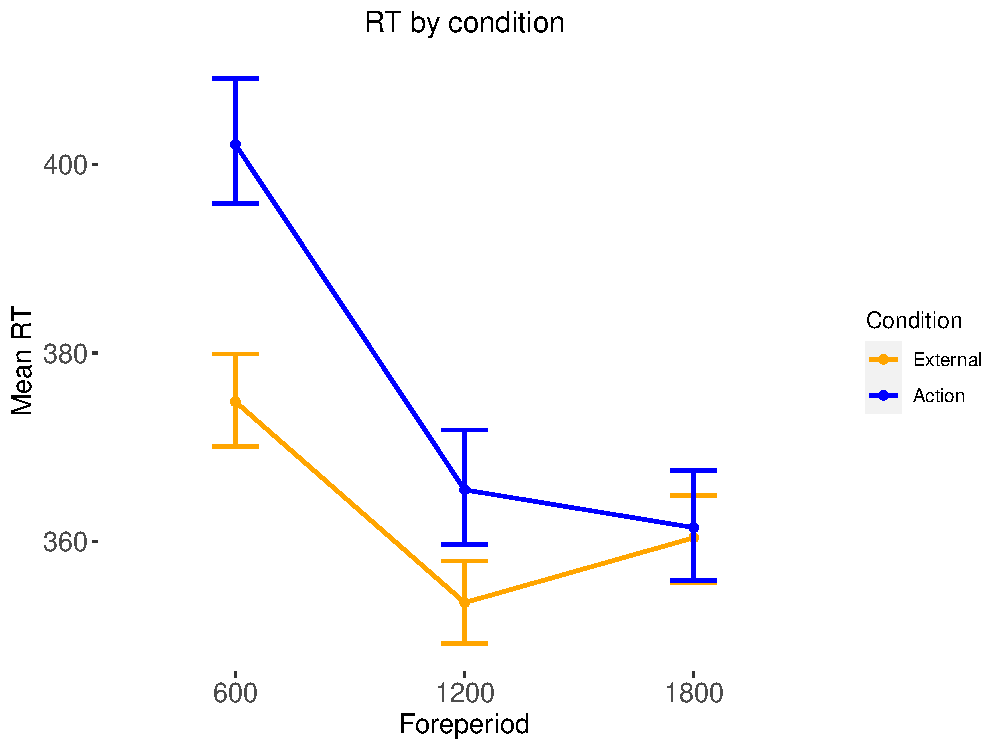
\includegraphics{RT_by_condition.pdf}
\centering
\end{figure}

Additionally, an interaction between FP\textsubscript{n} and FP\textsubscript{n-1} (\textit{F}(3, 101.92) = 11.33, \textit{p} < .001, $\eta_{p}^{2}$ = .250) indicates the presence of the classical asymmetric sequential effect, as shown in figure 3. Specifically, we found differences between levels of FP\textsubscript{n-1} for FP\textsubscript{n} = 600 ms, but no difference for FP\textsubscript{n} = 1200 ms. Crucially, however, we found no influence of condition on sequential effects, as indicated by a lack of a three-way interaction between condition, FP\textsubscript{n} and FP\textsubscript{n-1} (\textit{F}(3.16, 107.37) = 1.57, \textit{p} = .200, $\eta_{p}^{2}$ = 044).

\begin{figure}[h]
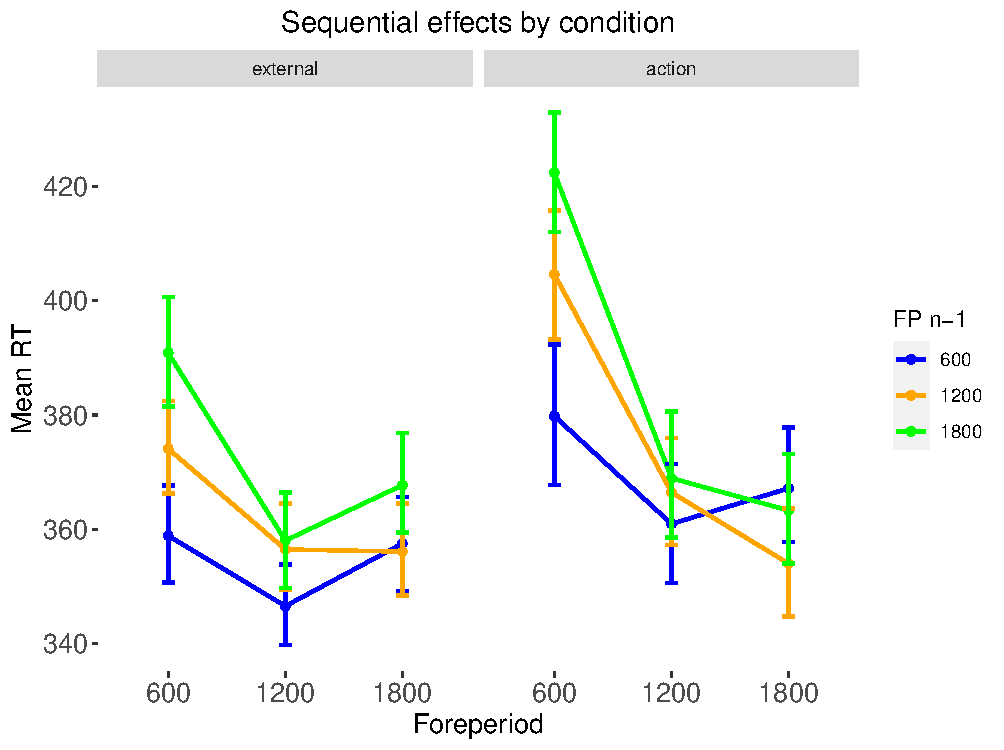
\includegraphics{SeqEff.pdf}
\centering
\end{figure}

Finally, we compared 

\subsection{Discussion}
The results of our first experiment suggest that voluntary actions influence temporal preparation.

However, a number of caveats must be made regarding the results. First, we observed a larger effect of actions on the shortest FP (600 ms). One possibility is that this was a result of a difficulty by participants in responding to stimuli presented shortly after the trial-start response in the action condition. Such a difficulty might be caused by a motor - psychological refractory period \cite{ittelstadt_evidence_2022} - or attentional - attentional blink \cite{yao_its_2023} - bottlenecks. Even though 

\section{Experiment 2}

The goal of this experiment was to replicate the effect observed in experiment 1 and remove the difference between go and no-go trials.

\subsection{Methods}

\subsubsection{Participants}
XXXXXXXX volunteers were recruited to participate in the study. All reported normal or corrected-to-normal vision and no history of neurological disorders, and none had any knowledge of the purpose of the study before the experiment. All participants read and signed an informed consent. XXXXXXX participants were removed from the analysis due to a large number of errors (> 10\% of trials), resulting in a final sample size of XXXXXXXX participants.

\subsubsection{Stimuli and procedure}
Experiment 2 used a similar design to experiment 1, with the following modifications. First, to remove the differences between go and no-go trials, we replaced the go/no-go task with a discrimination task. Second, to reduce the probability that the differences observed between external and action conditions were due to refractoriness of the response used to initiate the FP in the action condition, we used a longer duration for the shortest FP. Third, to run analysis with FP as a continuous predictor, we employed 4 FP durations instead of 3. Fourth, to emphasize the use of the WS as reference for temporal preparation instead of other events such as the response, ITI, or fixation cross onset, we employed an exponential distribution of ITI durations with XXXXXXXXXXX values \cite{jepma_temporal_2012}. %reference

Figure 1 shows an experimental trial. Each trial started with a black fixation cross presented at the center of the screen. The fixation cross remained on the screen for a period depending on the experimental condition. In the \textit{external} condition, the fixation cross remained on the screen for an interval of 1250-1750 ms (uniformly distributed), after which the warning signal (WS) was presented automatically. In the \textit{action} condition, the fixation cross remained on the screen until the participant pressed the space bar, which they could do whenever they desired. After either the fixation time or the voluntary action by the participant, the fixation changed color from black to green; this change was the WS and marked the onset of the FP. FP duration was either 600, 1200 or 1800 ms, and was pseudorandomly sampled from a uniform distribution in each trial, with the constraint the all durations were presented for an equal number of trials within a block. After the FP had elapsed, the fixation cross was replaced by the target: an imperative stimulus, which was either a go or no-go stimulus, as shown in Figure 1. Participants were instructed to press the space bar if they saw a go stimulus, or refrain from pressing any key if the saw a no-go stimulus. The target remained on the screen for 200 ms, and participants had up to 1000 ms to respond. After the response window, a blank screen was presented during a intertrial interval (ITI) drawn from a gaussian distribution with mean = 250 ms and sd = 25 ms. % min = 160 ms, max = 330 ms

\section{Experiment 3}



\printbibliography
%\bibliography{bibliography.bib}

\end{document}
